\documentclass[11pt]{article}

\usepackage[a4paper,margin=1in]{geometry}
\usepackage{setspace}
\usepackage{hyperref}
\usepackage{graphicx}
\usepackage{listings}
\usepackage{caption}
\usepackage{enumitem}

\setstretch{1.15}

\title{\textbf{From Image Classification to Threat Reasoning:}\\
Building an End-to-End Aircraft Identification and Decision Support Pipeline}

% \author{Jeevan Lowrence}
\date{}

\begin{document}
\maketitle

\begin{figure}[htbp]
    \centering
    
\includegraphics[width=0.8\textwidth]{images/LYFT_logo.png}
    % \caption{LYFT Logo}
    \label{fig:lyft_logo}
\end{figure}

\section*{Overview}

This project started with a simple question:

\emph{{How can we improve aircraft identification:} making it faster, more accurate, and enabling a more objective threat assessment—under operational time pressure??}

Inspired by how naval and air combat information officers operate in real-world settings, the goal evolved into building a system that does more than just classify an image. Instead, it aims to:

\begin{itemize}
    \item \textbf{Identify an aircraft from an image: } The type of aircraft.
    \item \textbf{Quantify confidence in that identification: } How sure are we that it is this aircraft.
    \item \textbf{Retrieve structured technical specifications: } What are the combat capabilities of this aircraft.
    \item \textbf{Reason about threat level under uncertainty: } Given the combat capabilities, how much of a threat does it  pose to ourself.
    \item \textbf{Recommend sensible next actions: } What's the best course of action given all the information we have(includes \textbf{HUMAN} in the loop here)
\end{itemize}

This document walks through how that system was built end-to-end, including what went wrong along the way.

\section*{High-Level Pipeline}

At a high level, the pipeline looks like this:

% \begin{enumerate}[label=\arabic*.]
%     \item Image input
%     \item Visual classification (Top-K)
%     \item Confidence-aware filtering
%     \item Aircraft specification lookup
%     \item Threat reasoning
%     \item Action recommendation
% \end{enumerate}

\vspace{0.5em}

\begin{figure}[htbp]
    \centering
    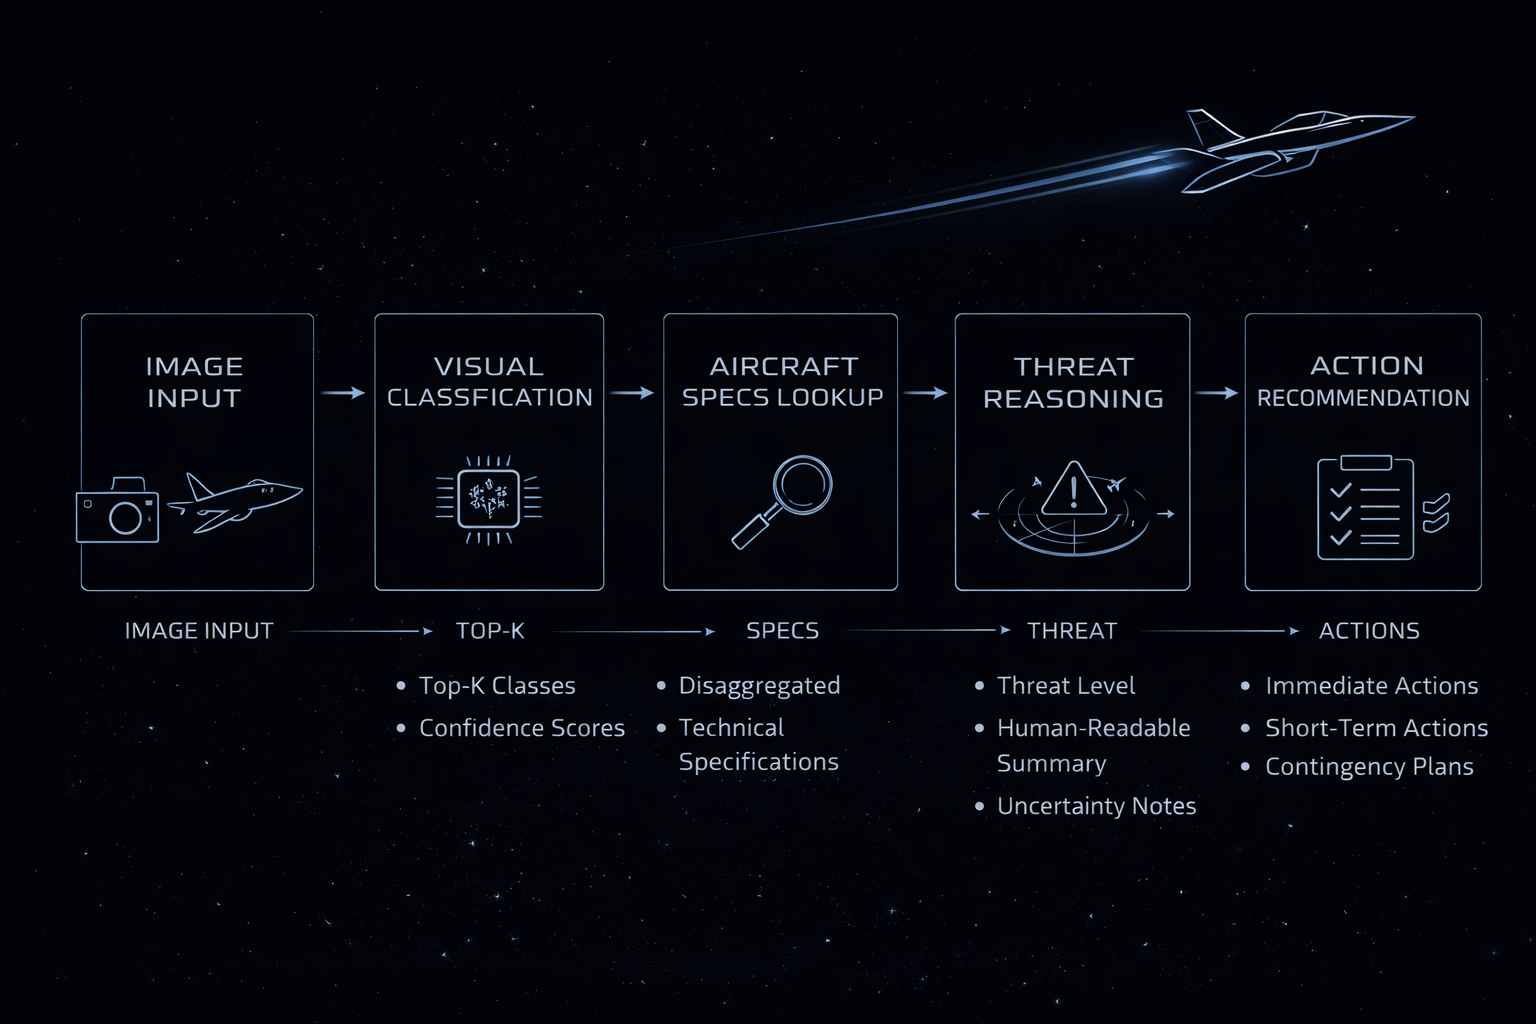
\includegraphics[width=0.8\textwidth]{images/pipeline.png}
    \caption{Operational Pipeline}
    \label{fig:pipeline}
\end{figure}


\section*{Dataset and Early Challenges}
Probably spent the most time over here (If not looped back and redid the data collection due to issues we will discuss later on). Used selenium to automate scraping from wikipedia headlessly because all the other options for looking up required api keys and unneccessary overcomplications and paywalls.

We collect the names of aircrafts and append it to a csv file and use the csv file then to collect the corresponding images after that to create our own dataset (\textit{In my head it was perfect, however given that I've enumerated the list of Challenges tells you something doesn't it?}). 

% \begin{enumerate}
%     \item Approach: Initial data collection just scraped the surface links from wikipedia where the approach was not to navigate too deep into the links and have too many dataset classes
%     \item Drawback: just got surface level aircraft list links like aircrafts from 1970s, aircrafts from 1980s etc.
% \end{enumerate}

% \begin{enumerate}[label=\textbf{Challenge \arabic*:}]
%     \item \textbf{Initial Wikipedia Scraping}
%     \begin{itemize}[leftmargin=1.5em]
%         \item[\textbf{Approach:}] Initial data collection just scraped the surface links from Wikipedia and append them to a csv file, where the approach was not to navigate too deep into the links and have too many dataset classes.
%         \item[\textbf{Drawback:}] Just got surface level aircraft list links like aircrafts from 1970s, aircrafts from 1980s, etc.
%         \item[\textbf{Solution:}] Used Ollama in the loop to assert whether the given page is a list of aircraft or aircraft itself.
%         \item[\textbf{Outcome:}] ~1700 aircraft classes, also \textbf{included explosions, accidents causing redundancy and noise in the dataset}.
%     \end{itemize}


%     \item \textbf{Revised Wikipedia Scraping for cleaning the csv}
%     \begin{itemize}[leftmargin=1.5em]
%         \item[\textbf{Approach:}] Refined the ollama query to filter and handle explosions, accidents, missing aircrafts and so on which caused redundancy and noise in the dataset.
%         \item[\textbf{Drawback:}] Link crawling got aggressive and started including prototypes, experimental weapons
%         \item[\textbf{Solution:}] Added filter for prototypes, experimental weapons as well using ollama.
%         \item[\textbf{Outcome:}] ~1300 aircraft classes, including \textbf{non-operational aircraft}.
%     \end{itemize}


%     \item \textbf{Image Collection}
%     \begin{itemize}[leftmargin=1.5em]
%         \item[\textbf{Approach:}] Naive Approach using common sites like wikimedia and image search results from google.
%         \item[\textbf{Drawback:}] Mostly contained non aircraft images and explosions, accidents had higher precedence rate.
%         \item[\textbf{Solution:}] Soft filtering using html scraping and alt text from the page source.
%         \item[\textbf{Outcome:}] ~800 aircraft classes.
%     \end{itemize}


%         \item \textbf{Insufficient Images}
%     \begin{itemize}[leftmargin=1.5em]
%         \item[\textbf{Approach:}] Most of the folders were Empty because of lack of documentation in early aviation era.
%         \item[\textbf{Drawback:}] Drastically reduced the class size.
%         \item[\textbf{Solution:}] Dropped aircrafts that had less images using a threshold because the previous models that had been trained did really bad.
%         \item[\textbf{Outcome:}] ~35 classes.
%     \end{itemize}
% \end{enumerate}

\begin{enumerate}[label=\textbf{Challenge \arabic*:}]
    \item \textbf{Initial Wikipedia Scraping}
        \begin{itemize}[leftmargin=1.5em]
            \item[\textbf{Approach:}] The initial data collection performed surface-level scraping of Wikipedia, extracting primary links and saving them to a CSV. This method was designed to avoid deep link navigation and an excessive number of dataset classes.
            \item[\textbf{Drawback:}] This resulted in only high-level category links (e.g., "aircraft from the 1970s," "aircraft from the 1980s") without differentiating between list pages and individual aircraft pages.
            \item[\textbf{Solution:}] Integrated Ollama into the pipeline to classify whether a given Wikipedia page represented a list of aircraft or a specific aircraft model.
            \item[\textbf{Outcome:}] Gathered approximately 1700 aircraft classes. However, the dataset included significant noise from unrelated pages such as aircraft accidents and explosions.
        \end{itemize}

    \item \textbf{Revised Wikipedia Scraping for Dataset Cleaning}
        \begin{itemize}[leftmargin=1.5em]
            \item[\textbf{Approach:}] Refined the Ollama query to explicitly filter out noise entries like accidents, explosions, and incomplete aircraft pages.
            \item[\textbf{Drawback:}] The more aggressive link crawling began including pages for \textbf{prototypes and experimental weapons}, which were not desired for the target operational dataset.
            \item[\textbf{Solution:}] Enhanced the Ollama filter to also exclude prototypes and experimental aircraft.
            \item[\textbf{Outcome:}] Reduced the dataset to roughly 1300 aircraft classes, though it still contained \textbf{non-operational aircraft}.
        \end{itemize}

    \item \textbf{Image Collection}
        \begin{itemize}[leftmargin=1.5em]
            \item[\textbf{Approach:}] Used a naive method to gather images from common sources like Wikimedia and Google search results.
            \item[\textbf{Drawback:}] The collected images were often irrelevant (non-aircraft), with a high prevalence of \textbf{accident and explosion scenes}.
            \item[\textbf{Solution:}] Implemented a soft filtering step using HTML scraping and the \textit{alt} text from page sources to better identify relevant images.
            \item[\textbf{Outcome:}] Successfully collected images for approximately 800 aircraft classes.
    \end{itemize}

    \item \textbf{Insufficient Images per Class}
        \begin{itemize}[leftmargin=1.5em]
            \item[\textbf{Approach:}] Many aircraft classes, particularly from the early aviation era, had few or no available images due to limited documentation.
            \item[\textbf{Drawback:}] This scarcity drastically reduced the usable number of classes for model training.
            \item[\textbf{Solution:}] Applied a minimum image threshold and removed all aircraft classes below it, as preliminary models trained on sparse data performed poorly.
            \item[\textbf{Outcome:}] Final dataset contained approximately \textbf{35 viable aircraft classes}.
    \end{itemize}
    
    \item \textbf{Final Data Quality and Structural Integrity}
    \begin{itemize}[leftmargin=1.5em]
        \item[\textbf{Approach:}] A final audit of the dataset revealed that one class (PN-1) contained significant noise and irrelevant images.
        \item[\textbf{Problem:}] Removing this class altered the label space, which caused a classifier head dimension mismatch in the trained model.
        \item[\textbf{Solution:}] The PN-1 class was purged, necessitating a complete model retrain from scratch.
        \item[\textbf{Outcome:}] This resulted in a final, clean dataset of 34 aircraft classes. The process underscored a critical lesson: any change to the label space has cascading effects and requires full retraining.
    \end{itemize}

    
    \end{enumerate}



    Once the dataset was fully vetted, it was then split 80:20 into train and val and metrics were measured for various models.



\section*{Model Training}

Several architectures were evaluated, including metric-learning approaches and transformer-based models. Ultimately, a fine-tuned EfficientNet variant provided the best balance between performance, stability, and inference speed for this use case.

Key techniques used:
\begin{itemize}
    \item \textbf{Class-balanced loss:}  Adjusts the loss function to account for imbalanced class distributions, preventing the model from being biased toward the majority classes.
    \item \textbf{Label smoothing} – Replaces hard one-hot labels with smoothed targets (e.g., 0.9 for the true class, 0.1 for others) to reduce model overconfidence and improve generalization.
    \item \textbf{Freeze / unfreeze scheduling} – Initially freezes the backbone layers to stabilize early training, then progressively unfreezes them to allow fine-tuning of deeper features.
    \item \textbf{Explicit overfitting diagnostics (train–val gap tracking)} – Systematically monitors the performance gap between training and validation sets to detect overfitting early and adjust regularization or training duration.
\end{itemize}

Despite achieving high training accuracy early, validation accuracy plateaued around 40\%. This gap was not ignored; it became a design constraint that influenced how much trust downstream reasoning should place on the classifier.

\newpage
\begin{figure}[htbp]
    \centering
    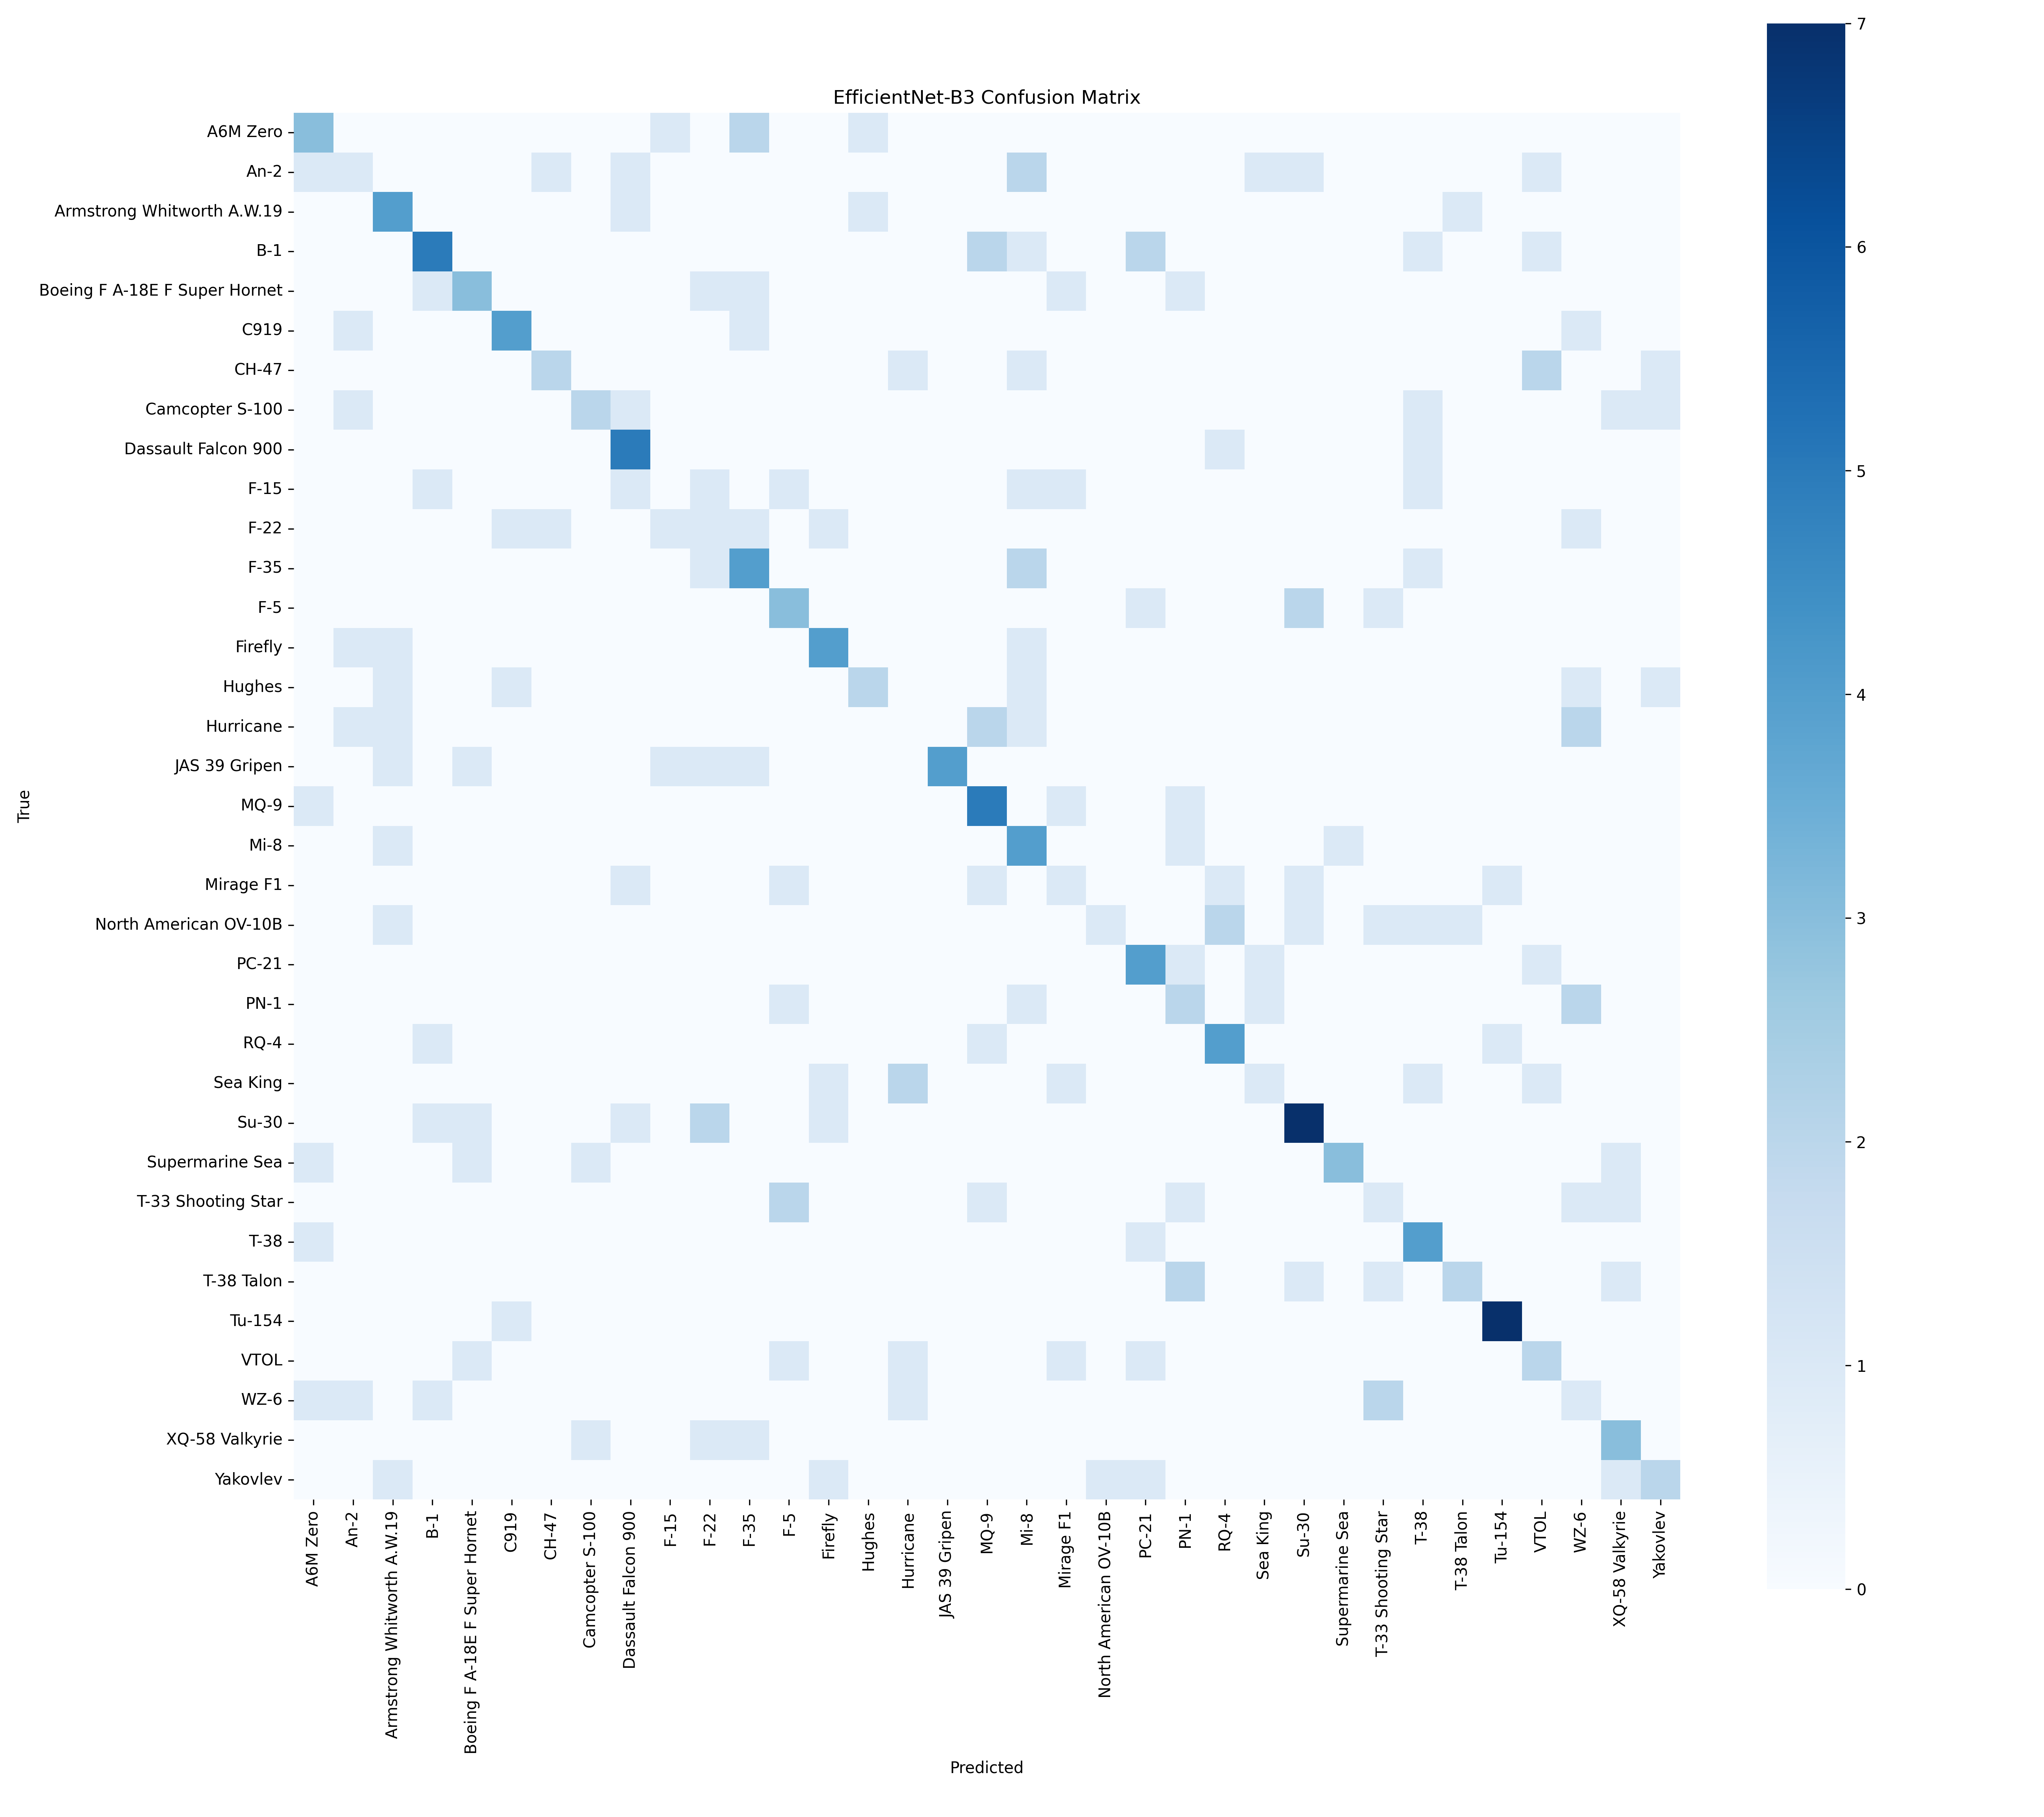
\includegraphics[width=1.3\textwidth]{images/confusion_matrix.png}
    \caption{EfficientNet Confusion Matrix}
    \label{fig:confusion matrix}
\end{figure}

\newpage

\section*{ Output }

\begin{figure}[htbp]
    \centering
    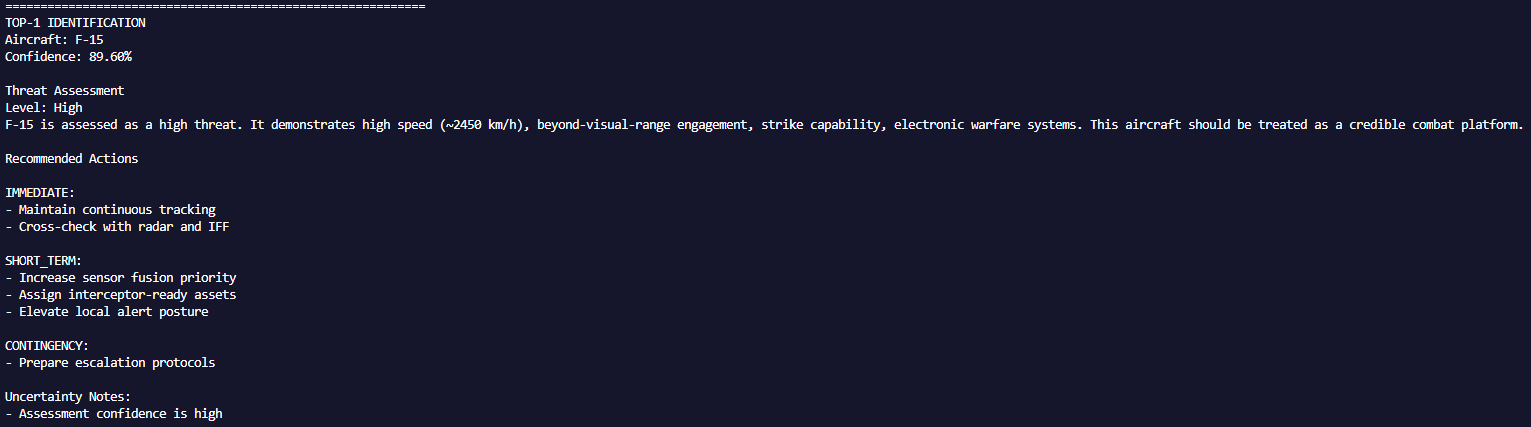
\includegraphics[width=1.3\textwidth]{images/output.png}
    \caption{Output for F22 Raptor}
    \label{fig:output}
\end{figure}

Note that this is the result for an F-22 raptor which got classified as an F-15 which is a different aircraft but since they're from the same family we'll take this as a win. 
Not to mention the fact that we only achieved 41\% accuracy with the model. 
We conclude that model performance cannot be improved further under the current conditions, as we are fundamentally limited by the small size and narrow scope of the available training data.

\section*{Top-K Classification Instead of Top-1}

Rather than relying on a single predicted class, the inference pipeline uses a Top-K approach. This decision was deliberate:

\begin{itemize}
    \item Real images are ambiguous
    \item Confidence matters more than correctness alone
    \item Downstream systems should degrade gracefully
\end{itemize}

Each Top-K output includes:
\begin{itemize}
    \item Aircraft name
    \item Confidence score
\end{itemize}

Only structurally valid predictions are accepted, preventing silent failures from malformed outputs.

\section*{Aircraft Specification Database}

To decouple vision from domain knowledge, aircraft specifications were extracted and stored separately.

For each aircraft:
\begin{itemize}
    \item A dedicated YAML file is generated
    \item Units are normalized numerically
    \item Capabilities are expressed as boolean flags
\end{itemize}

Example capability flags include:
\begin{itemize}
    \item Beyond-visual-range combat
    \item Strike capability
    \item Electronic warfare
    \item Stealth
\end{itemize}

This design allows the reasoning layer to remain model-agnostic and extensible.

\vspace{0.5em}
\noindent
\textbf{[Placeholder: Example YAML specification snippet]}

\section*{Threat Reasoning Under Uncertainty}

One of the most important lessons was that \textbf{missing data is normal}.

Specifications may be incomplete.
Classification confidence may be low.
Some aircraft may be poorly documented.

Instead of failing, the threat reasoning module:
\begin{itemize}
    \item Explicitly tracks uncertainty
    \item Adjusts threat labels based on confidence
    \item Emits explanatory summaries instead of raw scores
\end{itemize}

Threat levels are computed using interpretable heuristics such as speed, armament, and mission profile, not learned black-box scores.

Each assessment includes:
\begin{itemize}
    \item Threat level
    \item Human-readable summary
    \item Uncertainty notes
\end{itemize}

This mirrors how real analysts communicate risk.

\section*{Action Recommendation Layer}

On top of threat assessment sits an action recommender. This layer does not issue commands; it suggests sensible next steps based on doctrine-inspired logic.

Recommendations are grouped into:
\begin{itemize}
    \item Immediate actions
    \item Short-term actions
    \item Contingency preparations
\end{itemize}

For example, a high-confidence, high-threat identification may trigger suggestions such as continuous tracking, sensor fusion prioritization, or interceptor readiness.

\section*{Engineering Pitfalls and Fixes}

Several non-obvious issues emerged:
\begin{itemize}
    \item Multiprocessing failures on Windows due to missing \texttt{\_\_main\_\_} guards
    \item Model checkpoint incompatibility after class removal
    \item KeyErrors from mismatched dictionary contracts between modules
    \item NoneType propagation from partially populated specs
\end{itemize}

Each fix reinforced the importance of stable interfaces and defensive programming in multi-module systems.

\section*{Why This Matters}

This project is not about achieving state-of-the-art accuracy.

It is about:
\begin{itemize}
    \item Designing systems that reason under uncertainty
    \item Respecting the limits of machine perception
    \item Building pipelines that support humans, not replace them
\end{itemize}

The final system behaves less like a classifier and more like a junior analyst: confident when warranted, cautious when uncertain, and always explicit about its assumptions.

\section*{Next Steps}

Potential future extensions include:
\begin{itemize}
    \item Temporal tracking across multiple frames
    \item Multi-aircraft fusion
    \item Rules-of-engagement-aware recommendations
    \item Confidence-calibrated decision thresholds
\end{itemize}

\section*{Closing Thoughts}

Building this system required as much systems thinking as machine learning. Most of the work happened not in improving accuracy, but in making failures understandable and outputs actionable.

That, more than any metric, was the real objective.

\end{document}
